\documentclass{article}
\usepackage[utf8]{inputenc}

% biblatex (requires biber; sudo pacman -S biber)
\usepackage[style=authoryear-ibid]{biblatex} % biblatex
\addbibresource{"./content/bib/bib1.bib"}
\addbibresource{"./content/bib/bib2.bib"}

\usepackage{graphicx}
\graphicspath{ {./content/img/} }

\begin{document}

  Citation \autocite{gentry2009fully, Goodfellow-et-al-2016}

  Image:
  \begin{figure}[th!]
    \centering
    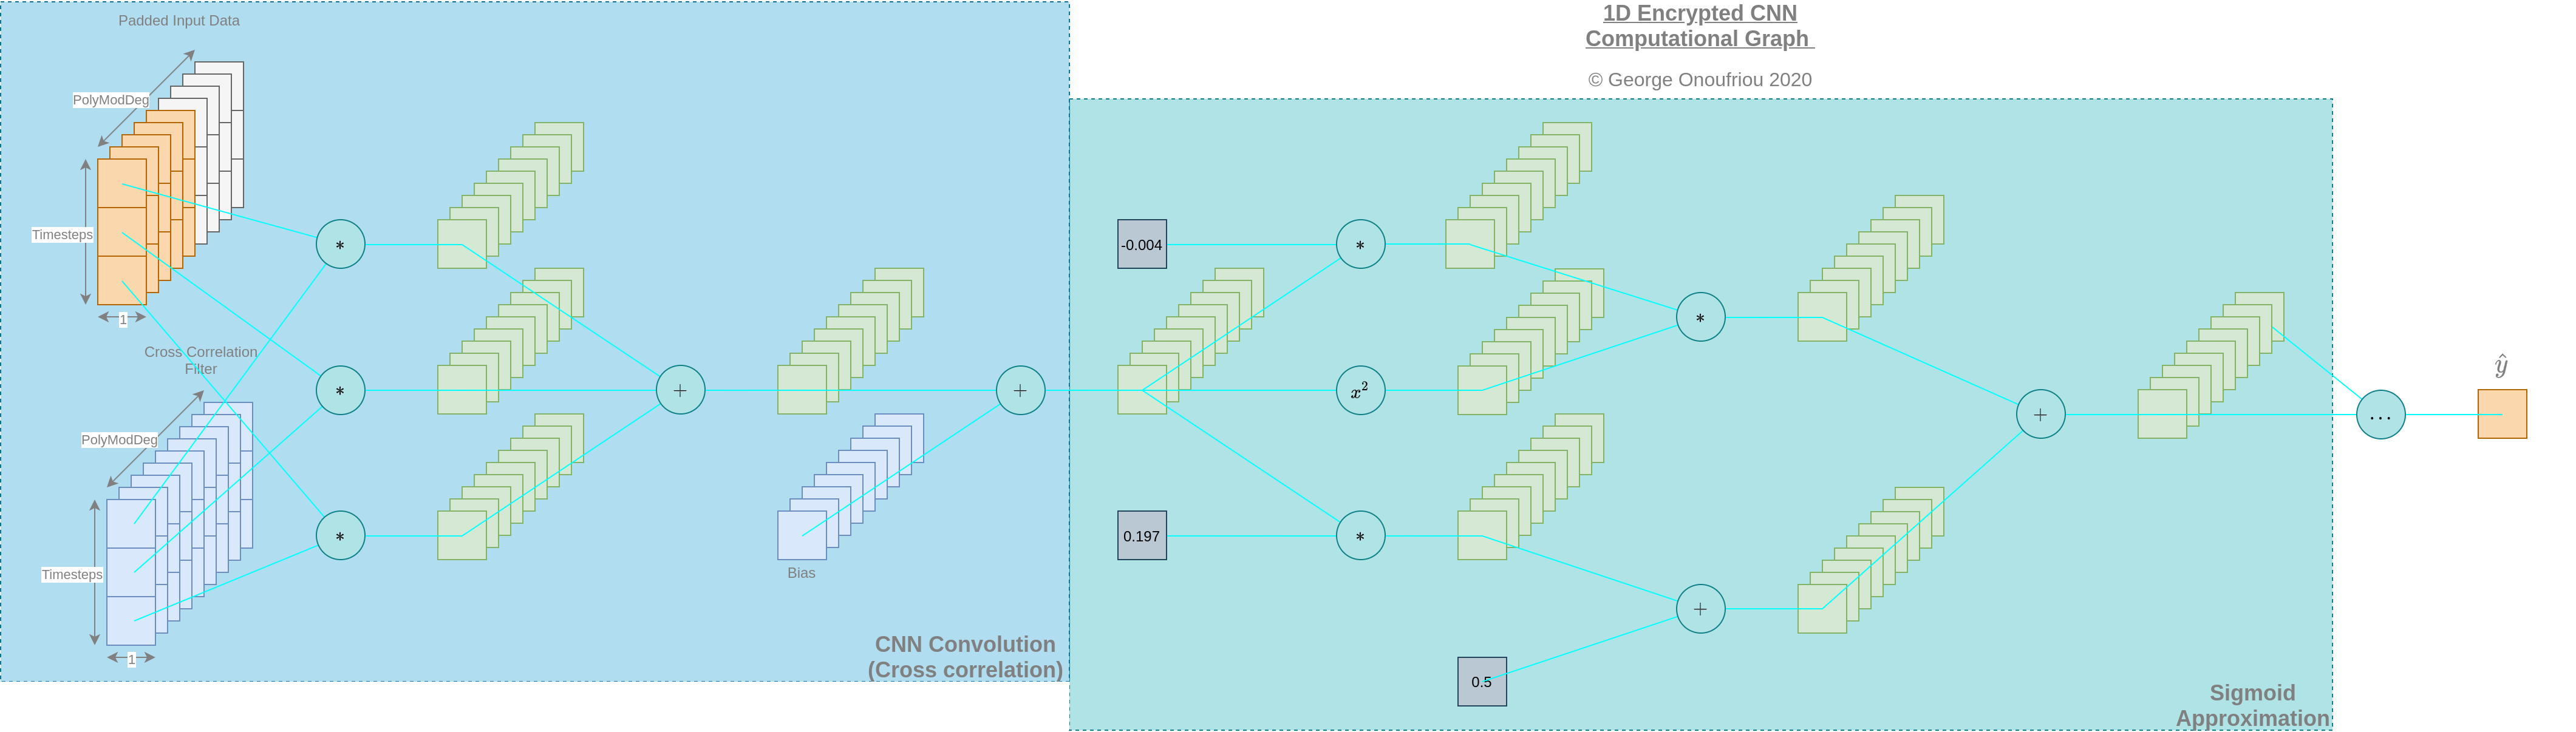
\includegraphics[width=\textwidth]{encrypted_cnn.png}
    \caption{Computational 1D CNN computational graph.}
    \label{fig:gan}
  \end{figure}

  Equations:

  \begin{equation}
    \label{sigmoid}
    \sigma(x) = \frac{1}{1+e^{-x}}
  \end{equation}

  \begin{equation}
    \label{sigmoid_approx}
    \sigma(x) \approx 0.5 + 0.197x + -0.004x^3
  \end{equation}

  \begin{equation}
    \label{cnn_activation}
    a^{<t>}=\sigma(w_{i}^{<t>}x^{<t>}+b_i^{<t>})
  \end{equation}

  \begin{equation}
    \label{gradient}
    \frac{df}{d\sigma} = (1-\sigma{x}) * \sigma{x}
  \end{equation}

  \begin{equation}
    \label{weight_update}
    % learning rate
    w_i^{j+1<t>} = w_i^{j<t>} - (l * \frac{df}{dw_i^{j<t>}})
  \end{equation}

  % % biblatex version
  \printbibliography

\end{document}
